\documentclass[a4paper, 11pt]{article}
\usepackage{graphicx}
\usepackage[utf8]{vietnam}
\usepackage{indentfirst}
\usepackage{longtable}
\usepackage{fdsymbol}
\usepackage{color}
\usepackage{biblatex}
\usepackage{fullpage}
\usepackage{blindtext}
\usepackage{hyperref}
\usepackage{multicol}
\usepackage{caption}
\usepackage{amsmath}
\usepackage[table]{xcolor}
\setcounter{MaxMatrixCols}{20}

\title{Bài tập tổng hợp cuối kỳ môn quản trị hệ thống}
\author{Kim Minh Thắng B2007210}

\begin{document}
\maketitle
\tableofcontents
\listoffigures
\listoftables

\section*{Mô tả bài tập}

Công ty Straw Hat chuyên kinh doanh hải sản có nhu cầu xây dựng hệ thống mạng cục bộ phục vụ cho công việc của công ty như sau:

\begin{minipage}{\linewidth}
    \captionsetup{type=figure}
    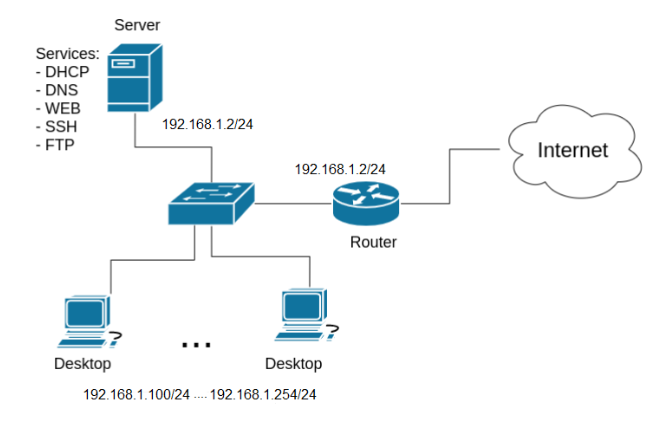
\includegraphics[width=12cm]{images/networks.png}
    \caption{Sơ đồ hệ thống mạng của công ty Straw Hat}
\end{minipage}

\section{Cài đặt và cấu hình Server/Desktop}

\subsection{(10\%) Sử dụng phần mềm VirtualBox cài đặt Server và Desktop:}

\begin{itemize}
    \item Tạo 1 NAT Network tên "QTHT" có địa chỉ mạng là 192.168.1.0/24. Tắt dịch vụ DHCP có sẵn trên NAT Network "QTHT". \hfill \\
          \begin{minipage}{\linewidth}
              \captionsetup{type=figure}
              \centering
              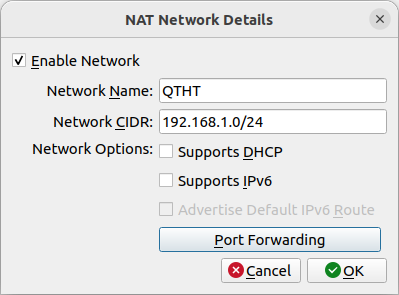
\includegraphics[width=8cm]{images/create-nat.png}
              \caption{Cấu hình NAT Network QTHT}
          \end{minipage}

          Để tắt dịch vụ DHCP mặc định của NAT Network trong VirtualBox, ta bỏ tích tùy chọn "Supports DHCP".

    \item Tạo 2 máy ảo với thông tin như sau: \hfill \\
          \begin{multicols}{2}
              \begin{minipage}{\linewidth}
                  \captionsetup{type=table}
                  \caption{Cấu hình máy Server}
                  \centering
                  \begin{tabular}{| p{.3\linewidth} | p{.4\linewidth} |}
                      \hline
                      \textbf{Hostname}         & Server                                                               \\
                      \hline

                      \textbf{Hệ điều hành}     & CentOS 9                                                             \\
                      \hline

                      \textbf{CPU / RAM / DISK} & 1core/2G/10G \newline Hoặc tùy chỉnh theo cấu hình máy của sinh viên \\
                      \hline

                      \textbf{Network}          & NAT Network \newline Name: "QTHT"                                    \\
                      \hline

                      \textbf{IP}               & 192.168.1.2                                                          \\
                      \hline

                      \textbf{Subnet mask}      & 255.255.255.0                                                        \\
                      \hline

                      \textbf{Gateway}          & 192.168.1.1                                                          \\
                      \hline

                      \textbf{DNS}              & 192.168.1.1                                                          \\
                      \hline
                  \end{tabular}
              \end{minipage}

              \begin{minipage}{\linewidth}
                  \captionsetup{type=table}
                  \caption{Cấu hình máy Desktop}
                  \centering
                  \begin{tabular}{| p{.3\linewidth} | p{.4\linewidth} |}
                      \hline
                      \textbf{Hostname}                                              & Desktop                                                              \\
                      \hline

                      \textbf{Hệ điều hành}                                          & Lubuntu 22.04, \newline hoặc bất kỳ hệ điều hành khác                \\
                      \hline

                      \textbf{CPU / RAM / DISK}                                      & 1core/2G/10G \newline Hoặc tùy chỉnh theo cấu hình máy của sinh viên \\
                      \hline

                      \textbf{Network}                                               & NAT Network \newline Name: "QTHT"                                    \\
                      \hline

                      \textbf{IP \newline Subnet mask \newline Gateway \newline DNS} & Cấu hình tự động sử dụng dịch vụ DHCP                                \\
                      \hline
                  \end{tabular}
              \end{minipage}
          \end{multicols}
          \begin{enumerate}
              \item \textbf{Server có cấu hình như sau:}
                    \begin{itemize}
                        \item Hệ điều hành: CentOS 9
                        \item CPU: 1 Core \textit{(Hình \ref{server-processor})}
                        \item Ram: 4GB \textit{(Hình \ref{server-ram})}
                        \item Disk: 20GB \textit{(Hình \ref{server-disk})}
                        \item Network: NAT Network "QTHT" \textit{(Hình \ref{server-network-1})}
                        \item IPv4: 192.168.1.2 \textit{(Hình \ref{server-network-2})}
                        \item Subnet mask: 255.255.255.0 \textit{(Hình \ref{server-network-2})}
                        \item Gateway: 192.168.1.1 \textit{(Hình \ref{server-network-2})}
                        \item DNS: 192.168.1.1 \textit{(Hình \ref{server-network-2})}
                    \end{itemize}

                    \begin{minipage}
                        {\linewidth}
                        \captionsetup{type=figure}
                        \centering
                        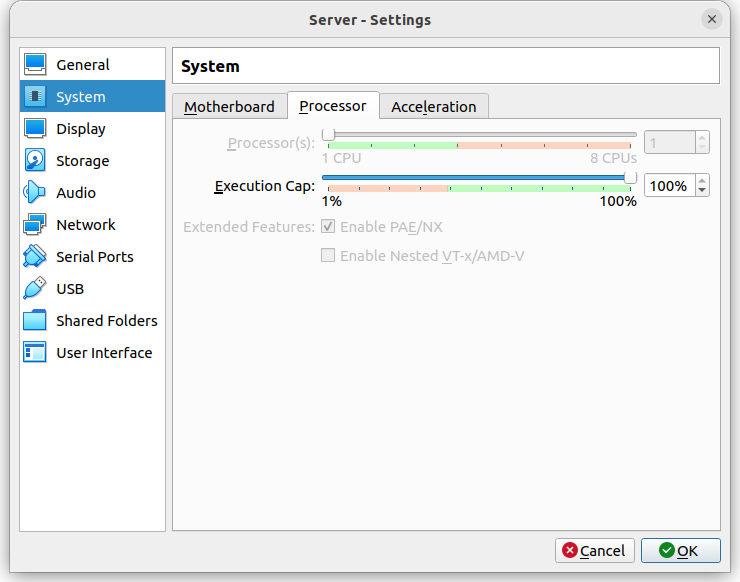
\includegraphics[width=12cm]{images/server-processor.png}
                        \caption{Số Core CPU cho Server}
                        \label{server-processor}
                    \end{minipage}

                    \begin{minipage}{\linewidth}
                        \captionsetup{type=figure}
                        \centering
                        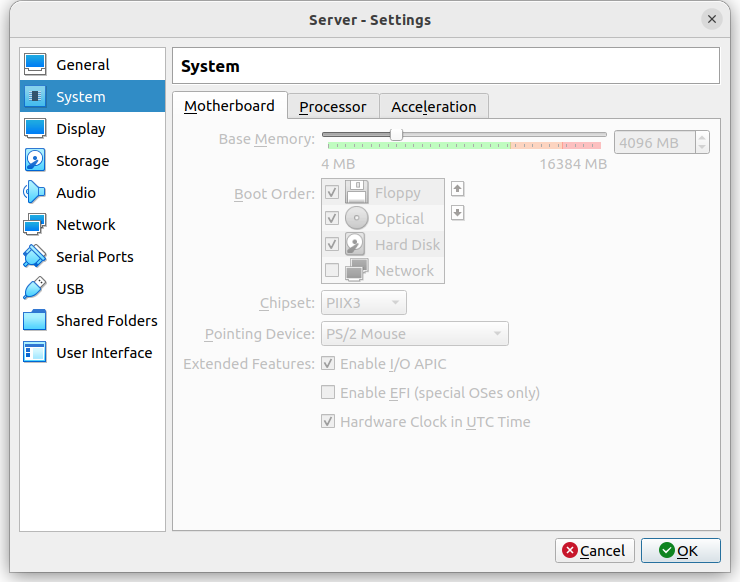
\includegraphics[width=12cm]{images/server-ram.png}
                        \caption{Dung lượng RAM cho Server}
                        \label{server-ram}
                    \end{minipage}

                    \begin{minipage}
                        {\linewidth}
                        \captionsetup{type=figure}
                        \centering
                        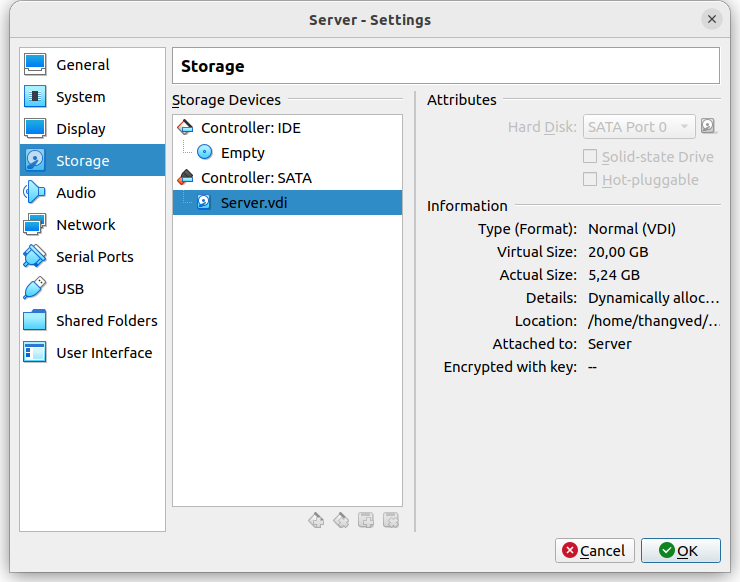
\includegraphics[width=12cm]{images/server-disk.png}
                        \caption{Dung lượng ổ cứng cho Server}
                        \label{server-disk}
                    \end{minipage}

                    \begin{minipage}
                        {\linewidth}
                        \captionsetup{type=figure}
                        \centering
                        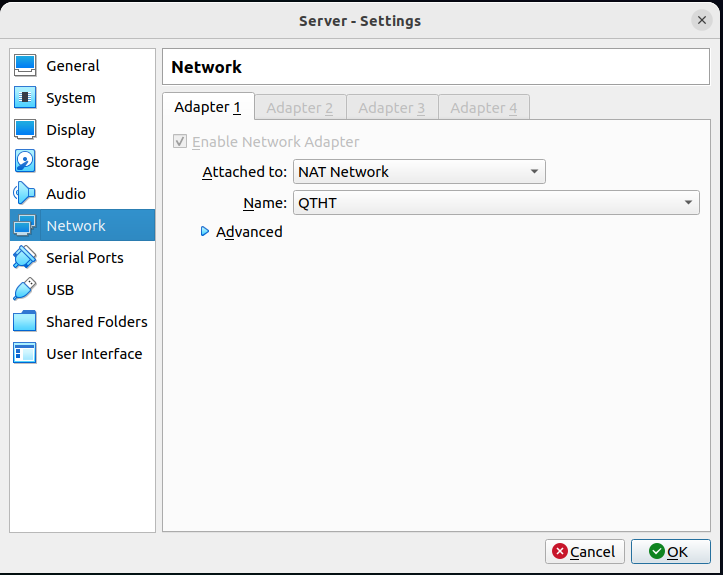
\includegraphics[width=12cm]{images/server-network-1.png}
                        \caption{Cấu hình mạng máy Server (1)}
                        \label{server-network-1}
                    \end{minipage}

                    \begin{minipage}
                        {\linewidth}
                        \captionsetup{type=figure}
                        \centering
                        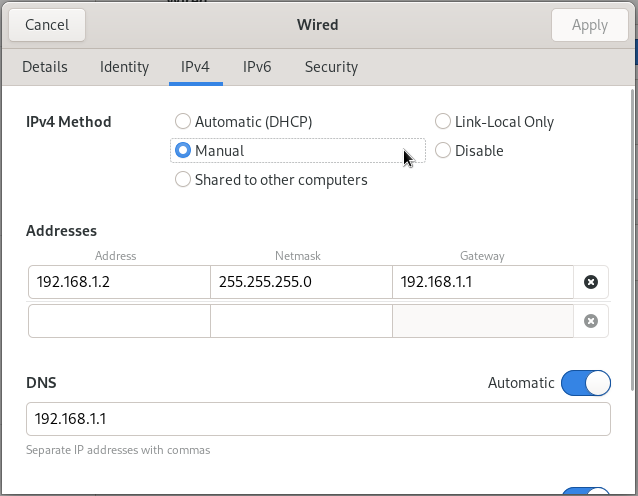
\includegraphics[width=12cm]{images/server-network-2.png}
                        \caption{Cấu hình mạng máy Server (2)}
                        \label{server-network-2}
                    \end{minipage}

              \item \textbf{Máy Desktop có cấu hình như sau:}
                    \begin{itemize}
                        \item Hệ điều hành: Lubuntu 22.04.3 LTS (Jammy Jellyfish)
                        \item CPU: 1 Core \textit{(Hình \ref{desktop-processor})}
                        \item Ram: 4GB \textit{(Hình \ref{desktop-ram})}
                        \item Disk: 20GB \textit{(Hình \ref{desktop-disk})}
                        \item Network: NAT Network "QTHT" \textit{(Hình \ref{desktop-network})}
                    \end{itemize}

                    \begin{minipage}
                        {\linewidth}
                        \captionsetup{type=figure}
                        \centering
                        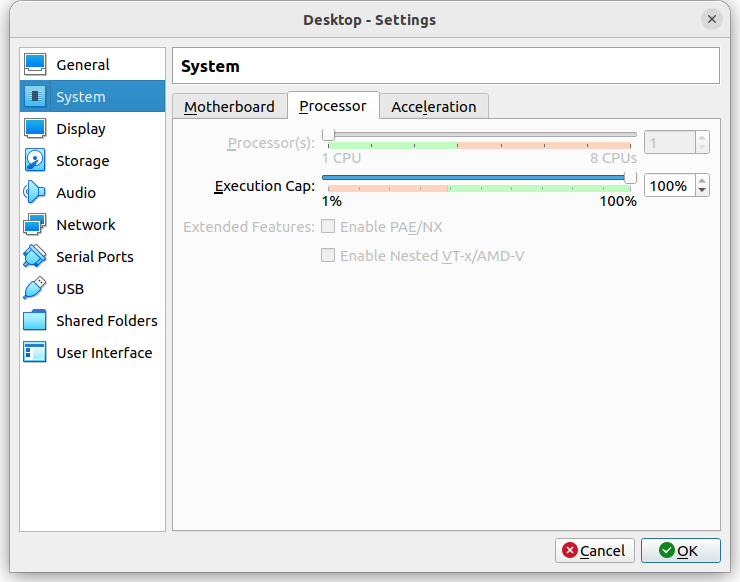
\includegraphics[width=12cm]{images/desktop-processor.png}
                        \caption{Số Core CPU cho máy Desktop}
                        \label{desktop-processor}
                    \end{minipage}

                    \begin{minipage}
                        {\linewidth}
                        \captionsetup{type=figure}
                        \centering
                        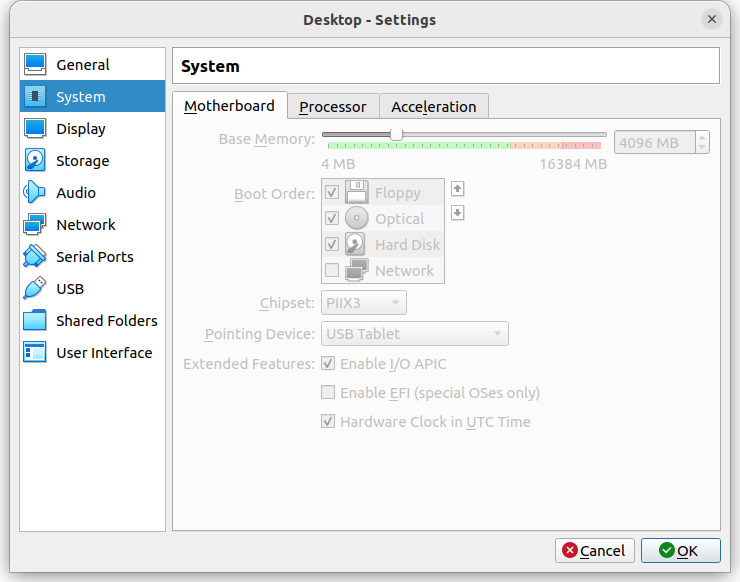
\includegraphics[width=12cm]{images/desktop-ram.png}
                        \caption{Dung lượng RAM cho máy Desktop}
                        \label{desktop-ram}
                    \end{minipage}

                    \begin{minipage}
                        {\linewidth}
                        \captionsetup{type=figure}
                        \centering
                        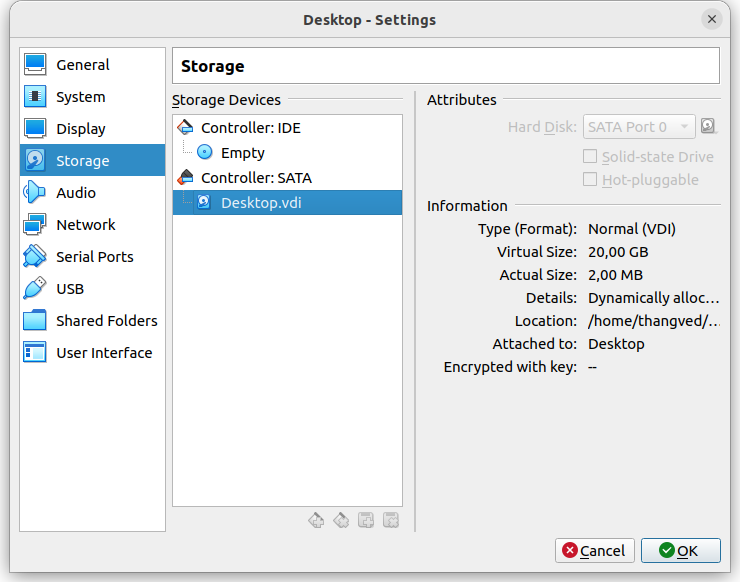
\includegraphics[width=12cm]{images/desktop-disk.png}
                        \caption{Dung lượng ổ đĩa cho máy Desktop}
                        \label{desktop-disk}
                    \end{minipage}

                    \begin{minipage}
                        {\linewidth}
                        \captionsetup{type=figure}
                        \centering
                        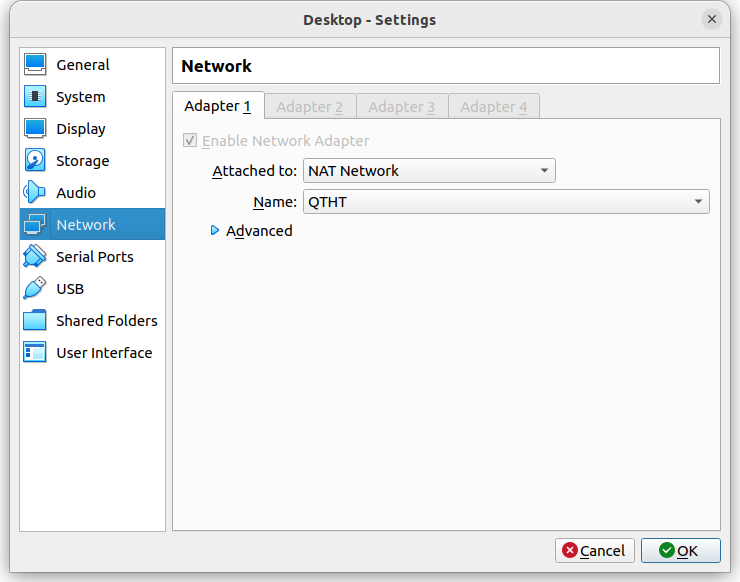
\includegraphics[width=12cm]{images/desktop-network.png}
                        \caption{Cấu hình mạng cho máy Desktop}
                        \label{desktop-network}
                    \end{minipage}
          \end{enumerate}
    \item Trong quá trình cài hệ điều hành CentOS 9, tạo 1 tài khoản với username là <Mã số sinh viên>; firstname và lastname là họ tên của sinh viên. Cấp quyền quản trị (sudo) cho tài khoản. Sử dụng tài khoản vừa tạo để thực hiện bài tập tổng hợp (không dùng tài khoản root).
    \item Tắt dịch vụ tường lửa trên Server. \hfill \\
          Để tắt tường lửa ta có thể sử dụng lệnh \texttt{systemctl} hoặc \texttt{service}.
          Ở đây ta sẽ sử dụng lệnh \texttt{systemctl} để làm việc này \textit{(xem Hình \ref{stop-firewalld}) và Hình \ref{disable-firewalld}}. \\

          \begin{minipage}
              {\linewidth}
              \captionsetup{type=figure}
              \centering
              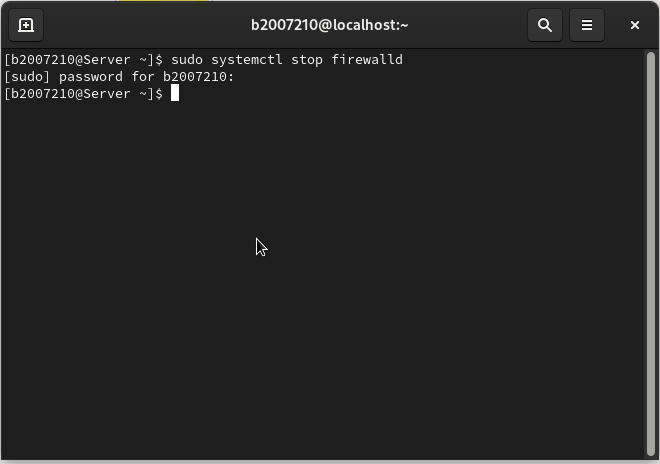
\includegraphics[width=12cm]{images/stop-firewalld.png}
              \caption{Dừng tường lửa bằng cách sử dụng \texttt{systemctl stop firewalld}}
              \label{stop-firewalld}
          \end{minipage}

          \begin{minipage}
              {\linewidth}
              \captionsetup{type=figure}
              \centering
              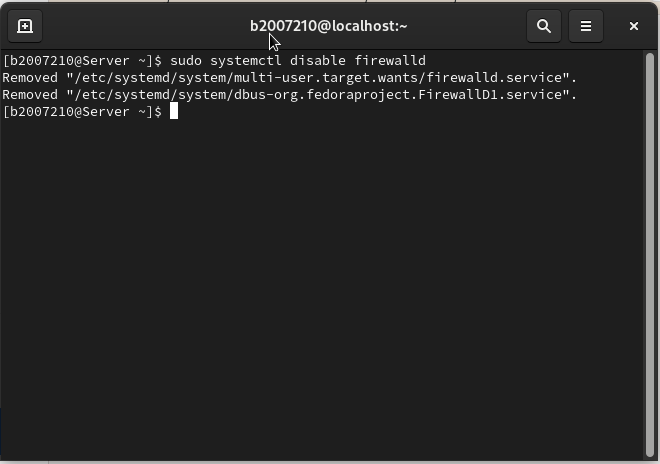
\includegraphics[width=12cm]{images/disable-firewalld.png}
              \caption{Ngăn tường lửa tự khởi động lại bằng cách sử dụng \texttt{systemctl disable firewalld}}
              \label{disable-firewalld}
          \end{minipage}

          Lệnh \texttt{systemctl stop firewalld} \textit{(Hình \ref{stop-firewalld})} dùng để dừng tường lửa ngay lập tức và lệnh \texttt{systemctl disable firewalld} \textit{(Hình \ref{disable-firewalld})} sẽ ngăn việc tường lửa tự khởi động lại sau khi reboot.
\end{itemize}

\subsection{(10\%) Tạo các người dùng và nhóm người dùng}

Để quản lý các bộ phận và người dùng trong công ty, hãy tạo các nhóm người dùng (group) và người dùng (user) trên server như sau. Cấp quyền sudo cho người dùng Nami.

\begin{longtable}{|c|c|c|c|c|c|}
    \caption{Danh sách người dùng và nhóm người dùng}              \\
    \hline
    STT & Họ tên  & Nhóm       & Username & Pasword & Mô tả        \\
    \hline

    1   & Luffy   & bangiamdoc & luffy    & luffy   & Giám đốc     \\
    \hline

    2   & Nami    & bangiamdoc & nami     & nami    & Phó giám đốc \\
    \hline

    3   & Zoro    & banhang    & zoro     & zoro    & Trưởng phòng \\
    \hline

    4   & Usopp   & banhang    & usopp    & usopp   & Nhân viên    \\
    \hline

    5   & Robin   & banhang    & robin    & robin   & Nhân viên    \\
    \hline

    6   & Sanji   & hanhchinh  & sanji    & sanji   & Trưởng phòng \\
    \hline

    7   & Chopper & hanhchinh  & chopper  & chopper & Nhân viên    \\
    \hline
\end{longtable}

\end{document}